\documentclass[10pt]{article}
\usepackage[polish]{babel}
\usepackage[utf8]{inputenc}
\usepackage[T1]{fontenc}
\usepackage{amsmath}
\usepackage{amsfonts}
\usepackage{amssymb}
\usepackage[version=4]{mhchem}
\usepackage{stmaryrd}
\usepackage{graphicx}
\usepackage[export]{adjustbox}
\graphicspath{ {./images/} }

\title{GIMNAZJUM }

\author{}
\date{}


\newcommand\Varangle{\mathop{{<\!\!\!\!\!\text{\small)}}\:}\nolimits}

\begin{document}
\maketitle
\begin{enumerate}
  \item Liczby \(a, b, c\) są dodatnie. Wykaż, że:
\end{enumerate}

\[
\frac{a}{a+1}+\frac{b}{(a+1)(b+1)}+\frac{c}{(a+1)(b+1)(c+1)}<1
\]

\begin{enumerate}
  \setcounter{enumi}{1}
  \item Ile dzielników ma liczba \(2^{2} \cdot 3^{5}+2 \cdot 3^{6}+2^{3} \cdot 3^{7}\) ?
  \item Oblicz sumę siedmiu zaznaczonych kątów:\\
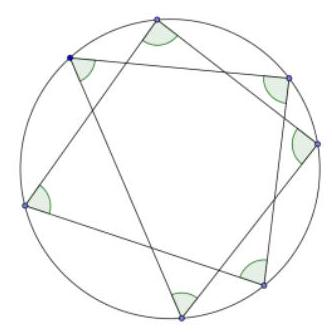
\includegraphics[max width=\textwidth, center]{2024_11_21_558747d4ea4aa1afd47eg-1}
\end{enumerate}

\section*{LICEUM}
\begin{enumerate}
  \item Uzasadnij, że dowolnej liczby naturalnej \(n\) :
\end{enumerate}

\[
(n+1)(n+2)(n+3) \cdot \ldots \cdot 2 n=2^{n} \cdot 1 \cdot 3 \cdot 5 \cdot \ldots \cdot(2 n-1)
\]

\begin{enumerate}
  \setcounter{enumi}{1}
  \item Wiadomo, że liczba \(a\) jest \(n\) razy większa od liczby \(b\), a suma liczb \(a\) i \(b\) jest \(m\) razy większa od ich różnicy. Znaleźć sumę \(m+n\), wiedząc, że \(m\) i \(n\) należą do liczb naturalnych.
  \item Dany jest pięciokąt wypukły \(A B C D E\), w którym \(B C=C D ; D E=E A\); \(\Varangle B C D=\Varangle D E A=90^{\circ}\). Wykaż, że z odcinków o długościach \(A C, C E, E B\) można zbudować trójkąt oraz wyznacz miary jego kątów, znając miarę \(\alpha\) kata \(A C E\) i miarę \(\beta\) kata \(B E C\).
\end{enumerate}

Rozwiązania należy oddać do piątku 19 czerwca do godziny 12.30 koordynatorowi konkursu panu Jarostawowi Szczepaniakowi lub swojemu nauczycielowi matematyki.

Na stronie internetowej szkoły w zakładce Konkursy i olimpiady można znaleźć wyniki dotychczasowych rund i rozwiązania zadań.


\end{document}